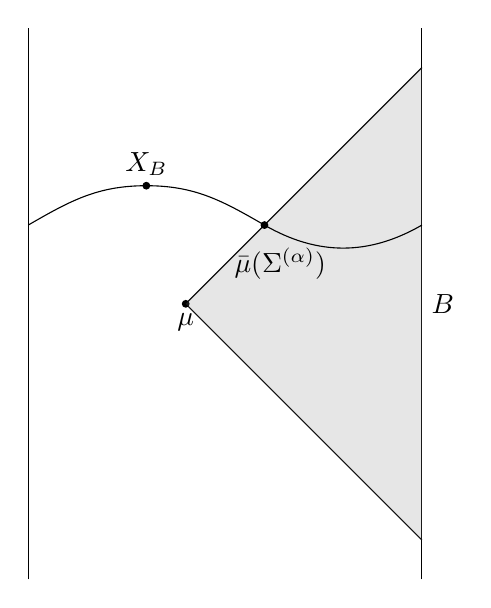
\begin{tikzpicture}
  \coordinate (bl) at (0, -0.5);
  \coordinate (tl) at (0, 6.5);
  \coordinate (tr) at (5, 6.5);
  \coordinate (br) at (5, -0.5);
  \coordinate (Sigl) at (0, 4);
  \coordinate (Sigr) at (5, 4);
  \coordinate[label=below:$\mu$] (mu) at (2, 3);
  \coordinate (owt) at (5, 6);
  \coordinate (owb) at (5, 0);
  \coordinate (sigrep) at (3, 4);
  \coordinate (xhrt) at (1.5, 4.5);

  \coordinate (blab) at (5, 3);

  \node at (mu) [circle, fill, inner sep=1pt]{};

  \draw (bl) to (tl);
  \draw (br) to (tr);


  \draw (mu) to (owt);
  \draw (mu) to (owb);
  \coordinate[label=right:$B$] (b) at (blab);
  \path[fill=gray, fill opacity=0.2] (mu) to (owb) to (owt) -- cycle;

  \onslide<3->{
    \draw (Sigl) to[out=30, in=180] (xhrt) to[out=0, in=150] (sigrep) to[out=-30, in=-150] (Sigr);
    \coordinate[label=above:$X_B$] (xlab) at (xhrt);
    \node at (xhrt) [circle, fill, inner sep=1pt]{};
  }

  \onslide<4->{
    \coordinate[] (xlab) at (sigrep);
    \node at (sigrep) [circle, label={[label distance=3pt, xshift=0.2cm] below:$\bar\mu(\Sigma^{(\alpha)})$}, fill, inner sep=1pt]{};
  }




\end{tikzpicture}
